%% Richard Wen
%% rwen@ryerson.ca


% *** INTRODUCTION ***


\section{Introduction} \label{introduction}

The wide availability of mobile devices have enabled millions of people to share online content, such as text, images, sound, and videos, from any location with wireless Internet connection. Social media platforms, such as Facebook \citep{Facebook:2017} and Twitter \citep{Twitter:2017}, are commonly used to share large amounts of online content in near real-time. This online content produces valuable sources of real-time locational data, known as geosocial media data, that may provide information on current real-world events such as traffic jams, natural disasters, disease spread, and terrorist attacks. 


% *** LITERATURE REVIEW ***


\section{Literature Review} \label{literature-review}

This section provides a literature review to provide background knowledge on current research related to the topic of \textit{"real-time geosocial media event detection and prediction"}. The paper selection process involved identifying reputable digital libraries using the Journal Impact Factor (JIF) measure \citep{Garfield:2006b}, followed by using automatic search queries to produce an initial list of potential papers. The potential papers were then further filtered by manual selection criteria to produce a list of selected papers for reviewing. Appendix \ref{appendix:literature-review-methods} provides details of the literature methods seen in Figure \ref{figure:litreview_process}.

\begin{figure}[!htb]
	\centering
	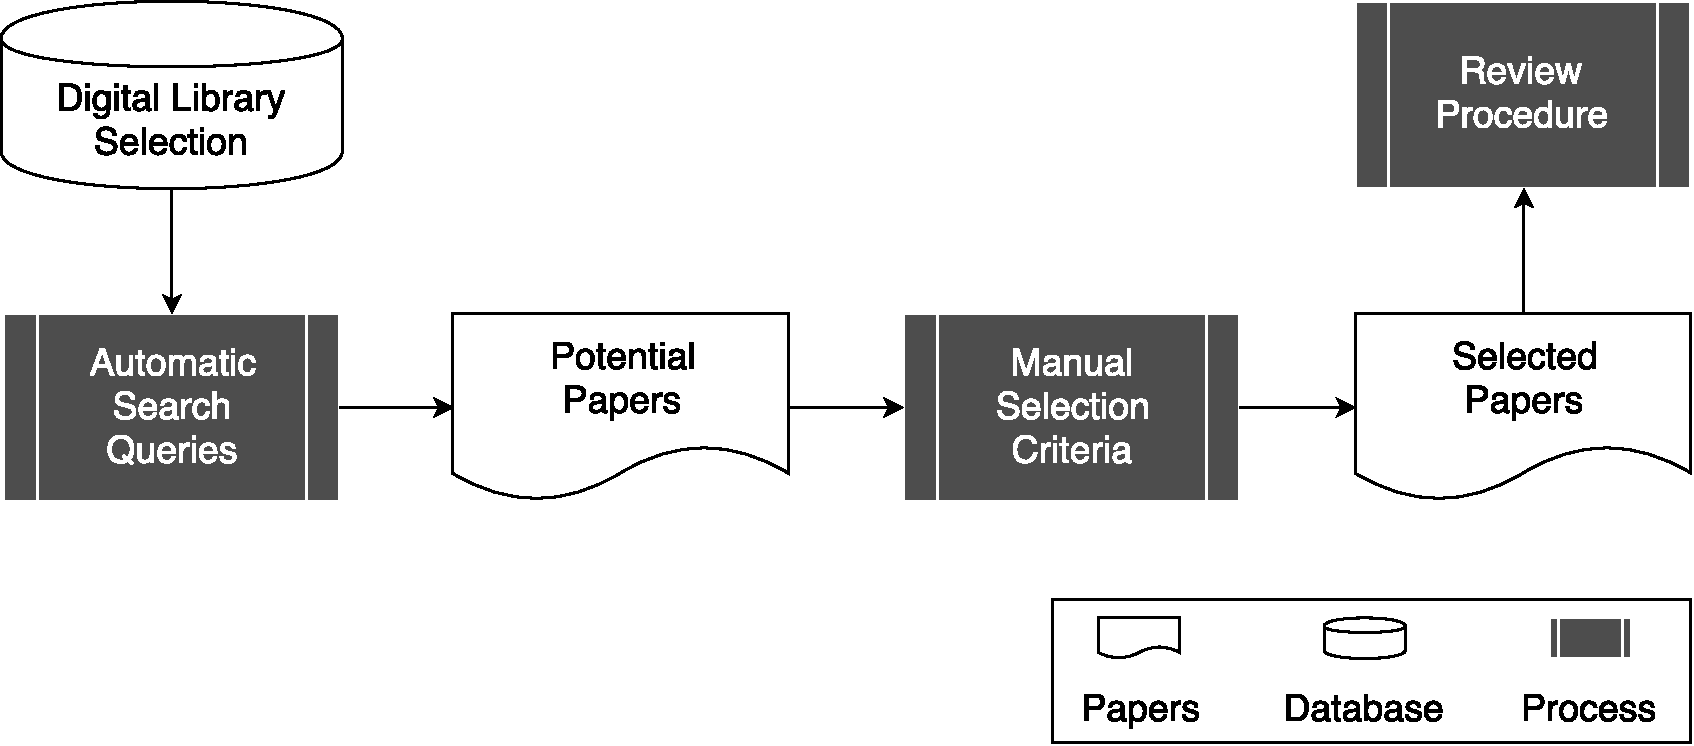
\includegraphics[width=6in]{litreview_process}
	\caption{\textbf{Literature Review Methods.}}
	\label{figure:litreview_process}
\end{figure}

\subsection{Event Detection} \label{event-detection-methods}

x

\subsection{Event Prediction} \label{event-detection-methods}

x

\subsection{Visualization} \label{event-detection-methods}

x